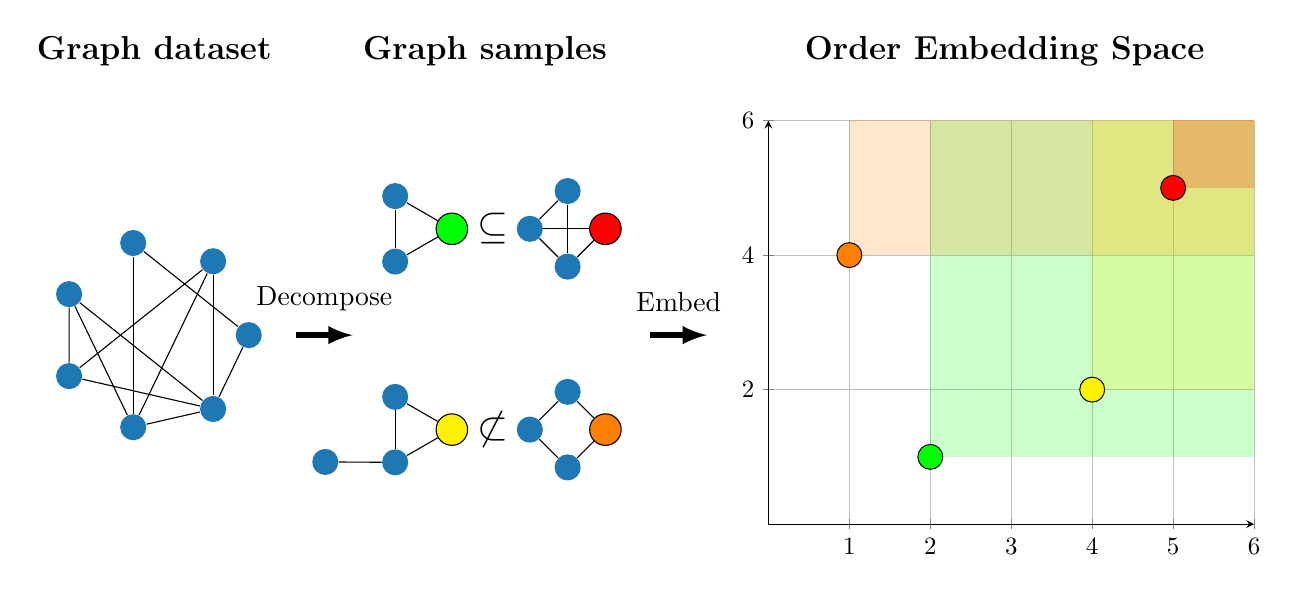
\begin{tikzpicture}[scale=0.6]
    \node at (-0.5, 6) {\large \textbf{Graph dataset}};
    \begin{scope}[shift={(-0.5,0)}]
      \draw
        (0.0:2) node[fill={rgb,255:red,31;green,119;blue,180}, minimum size=2mm, circle] (0){}
        (51.429:2) node[fill={rgb,255:red,31;green,119;blue,180}, minimum size=2mm, circle] (1){}
        (102.857:2) node[fill={rgb,255:red,31;green,119;blue,180}, minimum size=2mm, circle] (2){}
        (154.286:2) node[fill={rgb,255:red,31;green,119;blue,180}, minimum size=2mm, circle] (3){}
        (205.714:2) node[fill={rgb,255:red,31;green,119;blue,180}, minimum size=2mm, circle] (4){}
        (257.143:2) node[fill={rgb,255:red,31;green,119;blue,180}, minimum size=2mm, circle] (5){}
        (308.571:2) node[fill={rgb,255:red,31;green,119;blue,180}, minimum size=2mm, circle] (6){};
      \begin{scope}[-]
        \draw (0) to (2);
        \draw (0) to (6);
        \draw (1) to (4);
        \draw (1) to (5);
        \draw (1) to (6);
        \draw (2) to (5);
        \draw (3) to (4);
        \draw (3) to (5);
        \draw (3) to (6);
        \draw (4) to (6);
        \draw (5) to (6);
      \end{scope}
    \end{scope}
    \node at (6.5, 6) {\large \textbf{Graph samples}};
    \begin{scope}[shift={(2.5,0)}, scale=0.4]
      \draw[->, >=latex, line width=2pt] (0,0) --  node[label= above:Decompose] {} (3,0);
    \end{scope}
    
    \begin{scope}[shift={(8.25,2.25)}, scale=0.4]
      \draw
        (0.0:2) node[fill=red, minimum size=4mm, circle, draw, label] (1){}
        (90.0:2) node[fill={rgb,255:red,31;green,119;blue,180}, minimum size=2mm, circle] (3){}
        (180.0:2) node[fill={rgb,255:red,31;green,119;blue,180}, minimum size=2mm, circle] (4){}
        (270.0:2) node[fill={rgb,255:red,31;green,119;blue,180}, minimum size=2mm, circle] (6){};
      \begin{scope}[-]
        \draw (1) to (4);
        \draw (1) to (6);
        \draw (3) to (4);
        \draw (3) to (6);
        \draw (4) to (6);
      \end{scope}
    \end{scope}
    \begin{scope}[shift={(5,2.25)}, scale=0.4]
      \draw
        (0.0:2) node[fill=green, minimum size=4mm, circle, draw, label=right:\textbf{\Large $\subseteq$}] (1){}
        (120.0:2) node[fill={rgb,255:red,31;green,119;blue,180}, minimum size=2mm, circle] (4){}
        (240.0:2) node[fill={rgb,255:red,31;green,119;blue,180}, minimum size=2mm, circle] (6){};
      \begin{scope}[-]
        \draw (1) to (4);
        \draw (1) to (6);
        \draw (4) to (6);
      \end{scope}
    \end{scope}
    \begin{scope}[shift={(8.25,-2)}, scale=0.4]
      \draw
        (0.0:2) node[fill=orange, minimum size=4mm, circle, draw] (0){}
        (90.0:2) node[fill={rgb,255:red,31;green,119;blue,180}, minimum size=2mm, circle] (2){}
        (180.0:2) node[fill={rgb,255:red,31;green,119;blue,180}, minimum size=2mm, circle] (5){}
        (270.0:2) node[fill={rgb,255:red,31;green,119;blue,180}, minimum size=2mm, circle] (6){};
      \begin{scope}[-]
        \draw (0) to (2);
        \draw (0) to (6);
        \draw (2) to (5);
        \draw (5) to (6);
      \end{scope}
    \end{scope}
    \begin{scope}[shift={(5,-2)}, scale=0.4]
      \draw
        (0.0:2) node[fill=yellow, minimum size=4mm, circle, draw, label=right:{\textbf{\Large$\not\subset$}}] (1){}
        (120.0:2) node[fill={rgb,255:red,31;green,119;blue,180}, minimum size=2mm, circle] (4){}
        (240.0:2) node[fill={rgb,255:red,31;green,119;blue,180}, minimum size=2mm, circle] (6){}
        (200.0:5) node[fill={rgb,255:red,31;green,119;blue,180}, minimum size=2mm, circle] (7){};
      \begin{scope}[-]
        \draw (1) to (4);
        \draw (1) to (6);
        \draw (4) to (6);
        \draw (6) to (7);
      \end{scope}
    \end{scope}
    \begin{scope}[shift={(10,0)}, scale=0.4]
      \draw[->, >=latex, line width=2pt] (0,0) --  node[label= above:Embed] {} (3,0);
    \end{scope}
    \node at (17.5, 6) {\large \textbf{Order Embedding Space}};
    \begin{scope}[shift={(12.5,-4)}, scale=1.5]
        \begin{axis}[
            xmin=0, xmax=6,
            ymin=0, ymax=6,
            axis lines=center,
            grid=major,
        ]
                  
        % Shaded rectangular region for the red point
        \fill[green, opacity=0.2] (axis cs:2,1) rectangle (rel axis cs:2,1);
        
        % Shaded rectangular region for the red point
        \fill[orange, opacity=0.2] (axis cs:1,4) rectangle (rel axis cs:1,4);
        
        \fill[yellow, opacity=0.2] (axis cs:4,2) rectangle (rel axis cs:4,2);

        \fill[red, opacity=0.2] (axis cs:5,5) rectangle (rel axis cs:5,5);


        % Four points with big markers and labels
        \addplot[only marks, mark size=5pt, green, draw=black] coordinates {(2,1)};
        \node[red] at (axis cs:2,1) [above right] {};
        
        \addplot[only marks, mark size=5pt, orange, draw=black] coordinates {(1,4)};
        \node[orange] at (axis cs:1,4) [above right] {};
        
        \addplot[only marks, mark size=5pt, yellow, draw=black] coordinates {(4,2)};
        \node[blue] at (axis cs:5,2) [above right] {};
        
        \addplot[only marks, mark size=5pt, red, draw=black] coordinates {(5,5)};
        \node[orange] at (axis cs:4,5) [above right] {};
        
        \end{axis}     
    \end{scope}
  \end{tikzpicture}